\pdfoutput=1
\documentclass[11pt]{amsart}
\usepackage{amsmath,amssymb,amsthm,mathtools,mathrsfs}
\usepackage[margin=1.2in]{geometry}
\usepackage{graphicx,booktabs,adjustbox,tikz}
\usetikzlibrary{arrows.meta,positioning,calc}
\usepackage{xcolor,placeins}
\usepackage[colorlinks=true,linkcolor=blue,citecolor=blue,urlcolor=blue]{hyperref}
\hypersetup{pdfauthor={Bernd Johannes Wuebben},pdftitle={Hermitian--Yang--Mills flow at and beyond a stability wall}}
\setlength{\emergencystretch}{2em}
\newtheorem{theorem}{Theorem}[section]
\newtheorem{proposition}[theorem]{Proposition}
\newtheorem{lemma}[theorem]{Lemma}
\newtheorem{corollary}[theorem]{Corollary}
\theoremstyle{definition}
\newtheorem{definition}[theorem]{Definition}
\newtheorem{example}[theorem]{Example}
\newtheorem{question}[theorem]{Question}
\theoremstyle{remark}
\newtheorem{remark}[theorem]{Remark}
\newcommand{\CC}{\mathbb C}
\newcommand{\RR}{\mathbb R}
\newcommand{\ZZ}{\mathbb Z}
\newcommand{\PP}{\mathbb P}
\newcommand{\cO}{\mathcal O}
\newcommand{\cI}{\mathcal I}
\newcommand{\db}{\bar\partial}
\newcommand{\tr}{\operatorname{tr}}
\newcommand{\rk}{\operatorname{rk}}
\newcommand{\Hom}{\operatorname{Hom}}
\newcommand{\Coh}{\operatorname{Coh}}
\newcommand{\Vol}{\operatorname{Vol}}
\newcommand{\HYM}{\operatorname{HYM}}
\newcommand{\YM}{\operatorname{YM}}
\newcommand{\Gr}{\operatorname{Gr}}
\newcommand{\id}{\operatorname{id}}
\title[HYM flow at and beyond a stability wall]{Hermitian--Yang--Mills flow at and beyond\\ a stability wall}
\author{Bernd Johannes Wuebben}
\subjclass[2020]{53C07 (primary); 32G13, 58J35 (secondary)}
\keywords{Hermitian--Yang--Mills flow, stability wall, Harder--Narasimhan filtration, asymptotic phase, small eigenvalues}
\date{October 31, 2026\\This version: October 31, 2026}

\newcommand{\End}{\operatorname{End}}
\newcommand{\diag}{\operatorname{diag}}
\newcommand{\ad}{\operatorname{ad}}
\newcommand{\HH}{\mathsf H}
\newcommand{\cK}{\mathcal K}
\newcommand{\cR}{\mathcal R}
\newcommand{\cF}{\mathcal F}
\newcommand{\cD}{\mathscr D}

\newcommand{\cB}{\mathcal B}
\newcommand{\cN}{\mathcal N}
\newcommand{\cH}{\mathcal H}
\newcommand{\cM}{\mathcal M}
\newcommand{\cL}{\mathcal L}
\newcommand{\im}{\operatorname{im}}
\newcommand{\Lie}{\operatorname{Lie}}

\newcommand{\op}{\operatorname{op}}
\newcommand{\supp}{\operatorname{supp}}
\newcommand{\cQ}{\mathcal Q}
\newcommand{\cP}{\mathcal P}
\newcommand{\cV}{\mathcal V}

\begin{document}
\begin{abstract}
We prove all-time confinement and two-sided decay estimates for
Hermitian--Yang--Mills flow whose initial metric is a sufficiently small
transverse perturbation of a metric on a fixed finite-dimensional
invariant graph. The bundles are
small integrable deformations of a specified sum of four line bundles
on the product of three projective lines. At the stability wall the directed extension graph is acyclic
and connected; beyond it we treat a connected triangular class with locally
free Harder--Narasimhan line quotients. In a moving diagonal
presentation, the harmonic coefficients remain small although the
diagonal metric factors become unbounded. Their energy decays
reciprocally at the wall and crosses to exponential decay on the
unstable side, uniformly in the ratio of wall distance to initial
energy. This confinement yields an asymptotic phase relative to a
chosen invariant graph: each such initial metric selects a unique
reduced trajectory with exponentially decaying relative metric error.
The phase is continuously differentiable in the initial metric at
fixed bundle and polarization. At each fixed nearby unstable
polarization, subtracting the linear diagonal drift leaves a limiting
residual that is locally invertible in the three real diagonal initial
coordinates.
\end{abstract}

\maketitle


% Source: sections/01_introduction.tex
\section{Introduction}\label{sec:introduction}

Near a stable bundle, an equilibrium metric can confine a
Hermitian--Yang--Mills trajectory by metric order. At a stability
wall the corresponding extension may be strictly semistable,
and on the other side it may be unstable. The metric can then
leave every bounded set in its fixed holomorphic presentation.
Nevertheless, its extension coefficients in a moving diagonal
presentation can converge to zero. The distinction between
these two behaviors makes it possible to retain a quantitative
finite-dimensional description beyond the stable chamber.

This paper proves such a description for two classes of bundles
on $(\PP^1)^3$. The main step is an all-time energy estimate
that controls the coefficients without bounding the diagonal
metric factors. It yields a differentiable asymptotic phase,
relative spectral estimates and a common entry result for
prescribed initial metrics. On the strictly unstable side,
the reduced motion has a residual after subtraction of its
linear slope drift. That residual retains the three diagonal
initial conditions on a chosen invariant graph.

\subsection{The geometric classes}
The reference bundle is the sum of the four product line bundles
\[
 F_1=\cO(-2,-2,4),\quad F_2=\cO(1,-2,1),\quad
 F_3=\cO(-2,1,1),\quad F_4=\cO .
\]
The product polarization at the wall gives them equal slope.
Their full trace-free first deformation space has dimension
83, and their second deformation space has dimension five.
We use the complete analytic integrability equations on this
harmonic parameter space. Write $x_{ij}$ for a harmonic
coefficient in $\Hom(F_j,F_i)$; its directed support has the
arrow $j\to i$ when $x_{ij}\ne0$. The determinant-one diagonal
torus acts by $x_{ij}\mapsto g_i g_j^{-1}x_{ij}$.

At the wall, our domain consists of the nonzero integrable
tuples with connected acyclic support. Equivalently, these
are the connected integrable points in the torus nullcone:
zero belongs to the closure of their diagonal orbit.
Each resulting bundle is strictly semistable and has the
locally free Jordan--Hölder graded bundle
$E_0=\bigoplus_iF_i$. The domain includes all acyclic support
patterns in the full harmonic space. Acyclicity alone does
not impose the integrability equations.

For the unstable side, use the signed polarization path in
\eqref{eq:polarization} and write $l=-\tau$, with $\tau>0$.
We restrict to the five harmonic blocks
\[
 12,\quad13,\quad32,\quad24,\quad34 .
\]
This is a 32-dimensional harmonic subspace, subject to the
full integrability equations. Its order $1,3,2,4$ is
triangular. The associated subbundle flag has line quotients
whose centered mean curvatures, in that order, are
\[
 \tau,\quad0,\quad-2\tau/5,\quad-3\tau/5 .
\]
Thus it is the actual Harder--Narasimhan filtration for every
$\tau>0$. We require connected support, while allowing its
nonzero weights to be arbitrarily unequal. Composable arrows
are present: an explicit integrable example has a nonzero
quadratic correction in the endpoint block. The class is
therefore more than a sum of independent two-factor extensions.

The wall domain is larger than the triangular unstable domain.
Neither is asserted to exhaust all nearby semistable or
unstable bundles.

\subsection{Energy and the transition across the wall}
Fix one local parabolic invariant graph $\Psi(l,x)$ for the
metric flow. Its precise analytic properties are recalled
in Section~\ref{sec:setup}. On it the exact finite equation is
\[
 \dot x_{ij}=(\beta_i^\Psi-\beta_j^\Psi)x_{ij},\qquad
 \beta^\Psi(l,x)=b(l)-\mu_l(x)+O(|x|^4).
\]
Here $b(l)$ is minus the centered curvature of the split
reference, and $\mu_l(x)$ is the diagonal moment, the sum
of squared arrow norms times their incidence vectors.
This is the expansion of the exact field, not the definition
of a truncated evolution. Its trajectories reconstruct exact
Hermitian--Yang--Mills metric flows.

Let $q_l(x)=\sum_{ij}\|x_{ij}\|_l^2$ be the total harmonic
energy, with the spatial $L^2$ normalization specified below.
Along a trajectory put $q(t)=q_l(x(t))$ and $q_0=q(0)$.
For a graph trajectory at the wall, Theorem~\ref{thm:wall-energy}
gives
\begin{equation}\label{eq:intro-wall}
 \frac{q_0}{1+5q_0t}\ \le\ q(t)\
             \le\ \frac{q_0}{1+q_0t/5},
 \qquad t\ge0 .
\end{equation}
The diagonal coordinate $Y$, defined by $x=e^Yx_b$
for a fixed base tuple $x_b$, grows logarithmically in norm.
The decay of the coefficients thus coexists with divergence
of the metric.

On the unstable side, define
\[
 \mathcal L_{a,d}(q,t;\tau)=
 \frac{q e^{-a\tau t}}
 {1+\dfrac{dq}{a\tau}(1-e^{-a\tau t})}\quad(\tau>0),
 \qquad
 \mathcal L_{a,d}(q,t;0)=\frac{q}{1+dqt}.
\]
Theorem~\ref{thm:signed-energy} proves the two-sided bounds
\begin{equation}\label{eq:intro-transition}
 \mathcal L_{14/5,5}(q_0,t;\tau)
 \ \le\ q_{-\tau}(x(t))\
 \le\ \mathcal L_{2/5,1/5}(q_0,t;\tau).
\end{equation}
They hold for every future time, uniformly in the independent
scales $\tau$ and $q_0$. When $\tau\ll q_0$, they display a
reciprocal interval before exponential decay becomes decisive;
when $\tau$ is larger, the linear drift acts earlier. No
assumption orders these scales. The integral estimate
\begin{equation}\label{eq:intro-integral}
 \int_0^\infty q_{-\tau}(x(t))\,dt
       \le5\log\left(1+\frac{q_0}{2\tau}\right)
       \qquad(\tau>0)
\end{equation}
will determine the residual after subtracting that drift.

\subsection{The actual metric and its initial condition}
The energy estimates extend to metrics off the invariant
graph. Write a normalized initial metric in the form
$e^{Y_0\,*}(h_0e^{u_0})$ on the fixed bundle $d_{x_b}$.
The coefficient $x_0=e^{Y_0}x_b$ must be small, and the
complementary displacement
$v_0=u_0-\Psi(l,x_0)$ must be small in $h^{19/8}$, where
$h^s$ denotes the little H\"older space specified in
Section~\ref{sec:setup}.
There is no bound on $Y_0$, and no comparison between
the size of $v_0$ and the size of $x_0$.

Theorem~\ref{thm:local-tracking} selects a unique graph
trajectory $x_*(t)=e^{Y_*(t)}x_b$ with exponentially fast
relative metric tracking. If
$D=\|v_0\|_{h^{17/8}}$, its reconstructed metric $H_*(t)$
and the actual flow satisfy
\begin{equation}\label{eq:intro-tracking}
 e^{-CD e^{-4ct}}H_*(t)\le H(t)
                   \le e^{CD e^{-4ct}}H_*(t).
\end{equation}
The constants use the fixed complementary parabolic gap.
They are uniform in the absolute diagonal coordinates and
in all positive ratios of the three small finite eigenvalues.
The phase $Y_*(0)$ depends $C^1$ on the initial metric in
the stated relative coordinates, at each fixed bundle and
polarization. It is relative to the chosen graph, which
need not be canonical.

Let $\lambda_j(H(t))$ be the eigenvalues of the complex
trace-free Dolbeault Laplacian. Let $\nu_j(l,x)$ be the
three eigenvalues of the finite quadratic form
\[
 \xi\longmapsto\sum_{ij}\|x_{ij}\|_l^2|\xi_i-\xi_j|^2,
 \qquad \sum_i\xi_i=0,\qquad \|\xi\|^2=\sum_i|\xi_i|^2 .
\]
Connected support makes all three positive. Along the
selected trajectory,
\begin{equation}\label{eq:intro-spectra}
 \left|\log\frac{\lambda_j(H(t))}{\nu_j(l,x_*(t))}\right|
 \le Cq_l(x_*(t))+CD e^{-4ct}\quad(1\le j\le3),
 \qquad \lambda_4(H(t))\ge\gamma>0 .
\end{equation}
The coefficient term also tends to zero here. The largest
small eigenvalue is comparable to total energy; the two
smaller ones remain represented by the full finite form.
The total-energy bounds do not prescribe individual
asymptotic exponents for those modes.

Theorem~\ref{thm:prescribed} reaches this description from
every prescribed smooth determinant-normalized initial metric.
For a requested small normal tolerance it chooses one finite
restart, then coefficient, polarization and nearby-metric
neighborhoods. All their allowed flows satisfy the estimates
from that time onward. The initial-metric phase map remains
$C^1$. The restart is common on the chosen neighborhoods;
it may depend on the prescribed metric and requested tolerance.

\subsection{Residual drift and the graded limit}
For every fixed $\tau>0$, Theorem~\ref{thm:residual} proves
that the graph coordinate has a limit after its linear term
is removed:
\[
 Z_\infty=\lim_{t\to\infty}\bigl(Y(t)-b(-\tau)t\bigr),\qquad
 |Z_\infty-Y(0)|
       \le C\log\left(1+\frac{q_0}{2\tau}\right).
\]
For a fixed base tuple and graph, $Y(0)\mapsto Z_\infty$
is a $C^1$ local diffeomorphism on the three real diagonal
coordinates. The selected phase and the actual metric have
the same residual. Its initial-metric dependence is obtained
by composition with the phase map. These statements fix
$\tau>0$; neither the residual bound nor its derivative
bound is uniform at the wall.

There is also a direct quantitative connection estimate.
In the moving isometry
$U(t)=e^{u(t)/2}e^{Y(t)}$, Proposition~\ref{prop:graded-limit}
shows convergence to the split product connection $A_{0,l}$,
with
\[
 \|A(t)-A_{0,l}\|_{h^{9/8}}
 +\|F_{A(t)}-F_{A_{0,l}}\|_{h^{1/8}}
       \le C\bigl(q_l(x(t))^{1/2}+De^{-4ct}\bigr).
\]
The limit is the Hermitian--Einstein connection on the
Jordan--Hölder graded bundle at the wall and the Yang--Mills
connection on the Harder--Narasimhan graded bundle for
$\tau>0$. The estimate specifies the isometries and the
dependence on the evolving finite energy.

\subsection{Prior work and proof strategy}
Haiden, Katzarkov, Kontsevich and Pandit prove canonical
filtered asymptotics for metric flows on bundles over
curves, including linear slope drift and iterated logarithms
with bounded remainder \cite[Theorem 1.1 and Section 4.3]{HKKP18}.
Their discussion of polystable Harder--Narasimhan quotients
already exhibits exponentially decaying triangular coefficients.
Their metric-order comparison, unlike that curve asymptotic
theorem, applies in every complex dimension. We use this
comparison in the present threefold setting.

For semistable bundles with locally free Jordan--Hölder graded
object, Lam proves higher-dimensional finite-reduction and
asymptotic results. In the setting of his Section 8,
Proposition 8.6 gives bounded distance from the reduced flow,
and Theorem 8.7 supplies the equivariant Kuranishi description
\cite{Lam26}. Thus finite reduction itself, and the importance
of initial conditions in asymptotic descriptions, precede
the present results.

Smooth connection convergence modulo gauge to the
Harder--Narasimhan--Seshadri graded connection is also known
for each fixed polarization in our classes. Their graded
bundles are locally free, so the algebraic singular set in
the corrected \cite[Theorem 1.1(2)]{SibleyWentworth15} is empty.
Our final estimate gives a particular moving isometry and
a quantitative bound in the two specified Hölder norms.
It does not improve the regularity of that classical
qualitative convergence theorem.

The two-factor analysis in \cite[Theorem 5.4]{WuebbenFlow26}
already has a uniform profile through stable, wall and
unstable regimes. Its Sections 6 and 8 construct exact graph
flows and comparison after a prescribed-metric restart.
The common local reduction, the abstract differentiable
phase theorem and the signed nonstationary spectral estimate
needed here are established in \cite{WuebbenPhase26}.
Section~\ref{sec:setup} states their hypotheses and conclusions.
The full geometric family and its exact all-morphism statement
come from \cite[Sections 6 and 9]{WuebbenWall26}.

The new global argument begins with height coercivity on
acyclic support. It bounds the moment from below by total
energy uniformly in the support weights. On the triangular
unstable class, each allowed arrow also has a strictly
negative slope character. Together with the quartic
remainder of the exact field, these facts prove the
two-sided differential inequalities behind
\eqref{eq:intro-wall} and \eqref{eq:intro-transition}.

To use the local phase theorem with unbounded $Y$, we cut
off by coefficient energy, rather than by the size of $Y$.
Derivatives of the energy cutoff remain bounded because
every diagonal derivative of an arrow is bounded by its
own norm. Its finite Lipschitz constant is controlled by
$\tau+r^2$, with no condition on $\tau/r^2$. The perturbed
energy inequalities then remove the cutoff for both the
actual and selected trajectories. Cancelling their common
large diagonal factor gives the relative metric estimate.
An inverse coordinate estimate on convex energy sublevel
sets proves uniqueness without inverting a weak orbit
quadratic form.

Finally, for fixed $\tau>0$, the integral
\eqref{eq:intro-integral} makes the nonlinear correction
to linear drift integrable. The derivative of the finite
field along the trajectory is integrable as well. Its
variational matrix and inverse therefore converge, which
proves local invertibility of the residual map. These
arguments retain the initial condition while permitting
all finite spectral ratios to degenerate.

Sections~\ref{sec:wall} and \ref{sec:unstable} establish the
two geometric domains and their energy estimates.
Section~\ref{sec:phase} proves phase tracking and relative
spectra; Section~\ref{sec:entry} proves common entry from
prescribed metrics. Section~\ref{sec:residual} treats the
residual and the graded connection.

% Source: sections/02_setup.tex
\section{Geometry and the common local reduction}\label{sec:setup}

We state the finite reduction and analytic phase criterion with
the hypotheses needed below. The new global arguments will verify
those hypotheses without a bounded diagonal metric or an HE
equilibrium on the evolving bundle.

\subsection{The complete local deformation model}
On $X=(\PP^1)^3$, normalize the product Fubini--Study forms by
$\int_{\PP^1}\omega_i=1$, and set
\begin{equation}\label{eq:factors}
 \begin{gathered}
 F_1=\cO(-2,-2,4),\quad F_2=\cO(1,-2,1),\quad
 F_3=\cO(-2,1,1),\quad F_4=\cO,\\
 E_0=F_1\oplus F_2\oplus F_3\oplus F_4 .
 \end{gathered}
\end{equation}
Let $h_0,A_0,d$ be the product metric, Chern connection and
Dolbeault differential. Block $ij$ maps $F_j$ to $F_i$.
The determinant line is $\cO(-3,-3,6)$; its product metric
will remain fixed.

The reference harmonic space $V=H^1(X,\End_0E_0)$ has nine
nonzero blocks:
\[
 \begin{array}{c|ccc|ccc|ccc}
 ij&12&32&34&13&23&24&21&31&41\\ \hline
 \dim_{\CC}V_{ij}&8&8&4&8&8&4&8&8&27 .
 \end{array}
\]
Thus $\dim_{\CC}V=83$. The second cohomology has dimension
five, in block $14$. With the reference harmonic inclusion
$\iota$, projection $P_2$ and homotopy $K=d^*G$, the complete
reconstruction is
\begin{equation}\label{eq:reconstruction}
 a(x)=\iota x-K(a(x)^2),\qquad
 \kappa(x)=P_2(a(x)^2),\qquad d_x=d+a(x).
\end{equation}
It is analytic on a fixed coefficient ball. The operator $d_x$
is integrable exactly when all five components of $\kappa$
vanish, with all higher terms included. These facts and the
co-closed local model are proved in
\cite[Sections 6 and 9]{WuebbenWall26}.

Constant determinant-one complex diagonals act by
$(gx)_{ij}=g_i g_j^{-1}x_{ij}$. The reconstruction obeys
$a(gx)=ga(x)g^{-1}$ whenever both coefficient points lie in
its domain. Write
\[
 \mathfrak t=\{\xi\in\CC^4:\textstyle\sum_i\xi_i=0\},\qquad
 \mathfrak t_{\RR}=\mathfrak t\cap\RR^4,\qquad
 C_x\xi=((\xi_i-\xi_j)x_{ij})_{ij}.
\]
All nonconstant cross-Hom sections vanish: each nonzero
difference of the four degree triples has sum zero and a
negative component. The same co-closedness and complementary
coercivity used in \cite{WuebbenWall26} show that holomorphic
endomorphisms of a small integrable $d_x$ are exactly its
constant diagonal intertwiners.

\subsection{Polarizations, metrics and spectra}
Use the signed family
\begin{equation}\label{eq:polarization}
 \omega_l=h_1(l)\omega_1+h_2(l)\omega_2+\omega_3,\qquad
 h_1(l)=\left(1+\frac{7l}{30\pi}\right)^{-1},\quad
 h_2(l)=\left(1+\frac{l}{6\pi}\right)^{-1}.
\end{equation}
It is positive on an interval about zero. In the unstable
regime put $l=-\tau$, $\tau\ge0$. The centered slope demands are
\begin{equation}\label{eq:demand}
 b(l)=l(1,-2/5,0,-3/5).
\end{equation}
Thus the mean curvature of $F_i$, minus the average mean
curvature $\kappa_E(l)$, is $-b_i(l)$. The determinant metric
has constant mean curvature $4\kappa_E(l)$ for every $l$.

Divide squared spatial $L^2$ norms by $h_1h_2$. The resulting
measure and the diagonal zero-form mass $|\xi|^2=\sum_i|\xi_i|^2$
are fixed. Write
\begin{equation}\label{eq:energy}
 q_l(x)=\sum_{ij}\|x_{ij}\|_l^2,\qquad
 \mu_l(x)=\sum_{ij}\|x_{ij}\|_l^2(e_i-e_j).
\end{equation}
Relative to the reference norm $|x|$, the block weights are
$h_1^{-1}$ on $12,32,34$, $h_2^{-1}$ on $13,23,24$ and one
on $21,31,41$. They are uniformly positive. Put $q=q_0$ at
the wall.

Every flow below fixes $l$ and $d_{x_b}$ and solves
\begin{equation}\label{eq:flow}
 H^{-1}\dot H=-2(i\Lambda_lF_{d_{x_b},H}-\kappa_E(l)I),
                       \qquad \det H=\det h_0 .
\end{equation}
For positive metrics on the same bundle, $d_\infty(H_1,H_2)$
is the least $\eta$ such that
$e^{-\eta}H_2\le H_1\le e^\eta H_2$ pointwise.
Metric order is preserved by two exact solutions
\cite[Proposition 4.3]{HKKP18}. Global smooth existence follows
from \cite[Theorem 6.8.25]{Kobayashi87}, with its time equal
to twice our time.

The finite Hermitian form on $\mathfrak t$ is
\begin{equation}\label{eq:finite-spectrum}
 \langle\xi,L_{{\rm fin},l}(x)\xi\rangle
        =\|C_x\xi\|_l^2
        =\sum_{ij}\|x_{ij}\|_l^2|\xi_i-\xi_j|^2 .
\end{equation}
Its ordered eigenvalues are $\nu_1,\nu_2,\nu_3$, with zeros
included. The geometric eigenvalues $\lambda_j$ refer throughout
to $\bar\partial_{\End_0}^*\bar\partial_{\End_0}$ on complex
zero-forms, with complex multiplicity and no factor two.

\subsection{Exact sliced evolution and the graph}
Let $\mathcal V$ be the real bundle of $h_0$-Hermitian
trace-free endomorphisms, let $P_0$ be the fixed normalized
projection onto $\mathfrak t_{\RR}$, and put $Q_0=1-P_0$.
For nonintegral $s$, $h^s$ denotes the closure of smooth
sections in $C^s$. Define
\[
 \mathcal E_0=Q_0h^{3/8}(\mathcal V),\quad
 \mathcal E_1=Q_0h^{19/8}(\mathcal V),\quad
 \mathcal E_\alpha=Q_0h^{17/8}(\mathcal V),\quad \alpha=7/8.
\]
All these norms use the fixed background. Scale equivalent norms
so $\mathcal E_1\to\mathcal E_\alpha\to C^0$ have norm at most one.
For a complementary logarithmic metric $u$, set
\begin{equation}\label{eq:exact-field}
 \begin{aligned}
 \mathcal M(l,x,u)&=e^{u/2}i\Lambda_lF_{d_x,h_0e^u}e^{-u/2}
                                      -\kappa_E(l)I,\\
 S_u&=\frac{\sinh(\ad_u/2)}{\ad_u/2},\qquad
 C_u=\cosh(\ad_u/2),\qquad
 R(u)=P_0S_u^{-1}C_u|_{\mathfrak t_{\RR}},\\
 \beta(l,x,u)&=-R(u)^{-1}P_0S_u^{-1}\mathcal M(l,x,u).
 \end{aligned}
\end{equation}
The quotient has value one at zero, and $R(u)$ is positive
invertible. The compatible unitary connection defines this
curvature also on ambient nonintegrable coefficients.

We use the following precise consequences of
\cite[Sections 3, 4 and 7]{WuebbenPhase26}. They hold on a common
signed parameter interval and coefficient neighborhood.
For any fixed finite $m\ge6$ one can choose a $C^m$ invariant
graph $\Psi(l,x)\in\mathcal E_1$ with
\begin{equation}\label{eq:graph-bounds}
 \Psi(l,0)=D_x\Psi(l,0)=0,\qquad
 \|\Psi(l,x)\|_{\mathcal E_1}\le C|x|^2,\qquad
 \|D_x\Psi(l,x)\|\le C|x|.
\end{equation}
Its exact reduced vector field is $\beta^\Psi(l,x)=\beta(l,x,\Psi(l,x))$,
with expansion
\begin{equation}\label{eq:field-jet}
 \beta^\Psi(l,x)=b(l)-\mu_l(x)+\mathcal R_l(x),\qquad
 |D_x^j\mathcal R_l(x)|\le C|x|^{4-j}\quad(0\le j\le2).
\end{equation}
Fix a uniform constant $C_E$ such that
$|\mathcal R_l(x)|\le C_Eq_l(x)^2$ on this signed neighborhood;
the equivalence of $q_l(x)$ and $|x|^2$ gives such a constant.
The equation and reconstruction are
\begin{equation}\label{eq:finite-flow}
 \dot Y=\beta^\Psi(l,e^Yx_b),\qquad x=e^Yx_b,\qquad
 H_*=e^{Y\,*}(h_0e^{\Psi(l,x)}).
\end{equation}
Every integrable trajectory staying in the graph domain gives
an exact solution of \eqref{eq:flow} on $d_{x_b}$.
The graph is fixed from now on; it is not required to be
positive-diagonal equivariant. The equivariance of $a$ is what
identifies the holomorphic bundle in this reconstruction.

Off the graph the exact slice has the form
\begin{equation}\label{eq:normal-system}
 \dot x=C_x\beta(l,x,u),\qquad
 \dot u=-A_lu+\mathcal N_l(x,u),\qquad
 A_l=2L_l|_{Q_0},\quad
 L_l=\tfrac12(\Delta_{\partial,l}+\Delta_{\bar\partial,l}).
\end{equation}
The first-jet maps extend smoothly from
$V\times Q_0h^{13/8}$ to the finite space and $\mathcal E_0$.
For every signed $l$,
$D_u\beta(l,0,0)=0$ and $D_{(x,u)}\mathcal N_l(0,0)=0$.
The common-domain semigroup satisfies
\begin{equation}\label{eq:semigroup}
 \|e^{-tA_l}\|_{\mathcal E_\alpha\to\mathcal E_\alpha}
        \le Me^{-\sigma_0t},\qquad
 \|e^{-tA_l}\|_{\mathcal E_0\to\mathcal E_\alpha}
        \le M(1+t^{-7/8})e^{-\sigma_0t}.
\end{equation}
The constants are uniform. The principal operator includes the
signed curvature commutator; no extra linear $b\,u$ term is
to be added to \eqref{eq:normal-system}.

The same reference harmonic orthogonality and complementary
coercivity give, for every small integrable $x$ and signed $l$,
\begin{equation}\label{eq:static-spectrum}
 (1-C|x|^2)\nu_j(l,x)\le\lambda_j(h_0,x;l)
       \le(1+C|x|^2)\nu_j(l,x),\quad 1\le j\le3,\qquad
 \lambda_4\ge\gamma_0 .
\end{equation}
The kernel is exactly the constant $\ker C_x$.
Changing to $h_0e^{\Psi(l,x)}$ preserves the relative order
$O(q_l(x))$. The proof in \cite[Lemma 7.1]{WuebbenPhase26}
eliminates only the uniformly coercive complement, before
min--max on the three finite directions. It uses positivity
of the product coefficients and bounds by $C|l|$, so its
signed scope does not follow merely by extrapolating an
estimate stated on the stable side.

\subsection{The analytic phase criterion}
For clarity we also state the analytic input
\cite[Proposition 4.1]{WuebbenPhase26}. Suppose
\[
 \dot Y=f(Y)+h(Y,v),\qquad \dot v=-A_lv+F(Y,v)
\]
has a bounded $C^2$ reduced vector field with bounded second derivative
and sufficiently small $\|Df\|_\infty$. On a fixed open normal
ball in $\mathcal E_\alpha$, suppose $h,F$ are $C^2$ with
uniformly bounded derivatives, vanish at $v=0$, and satisfy
\[
 \|D_vh\|+\|D_vF\|\le\epsilon,\qquad
 \|D_Yh\|+\|D_YF\|\le K\|v\|_{\mathcal E_\alpha}.
\]
Here $\epsilon$ is sufficiently small relative to
\eqref{eq:semigroup}. If also
$\|D_vh\|\le K(a+\|v\|_{\mathcal E_\alpha})$, then for small
initial normal size $D$ there is a selected solution of the reduced equation with
\begin{equation}\label{eq:phase-input}
 \|v(t)\|_{\mathcal E_\alpha}\le CD e^{-4ct},\qquad
 |Y_*(t)-Y(t)|\le C(a+D)D e^{-4ct},\qquad c=\sigma_0/8 .
\end{equation}
Its phase $\Pi(Y_0,v_0)$ is $C^1$ with uniform derivative bounds,
equals $Y_0$ on graph data, and obeys
$\|D_{v_0}\Pi\|\le C(a+\delta)$ on $\|v_0\|<\delta$.
It is obtained as $\lim_{t\to\infty}\phi_{-t}(Y(t))$ for
the complete reduced flow $\phi$. The proof differentiates
this improper limit using integrable variation estimates.
It neither assumes an equilibrium nor inverts a finite rate.
The new work below is to produce a global reduced vector field to which
this criterion applies, then remove its cutoff on both trajectories.

% Source: sections/03_wall.tex
\section{The integrable nullcone at the wall}\label{sec:wall}

At $l=0$ the reduced vector field has no constant drift. Its total
coefficient energy is coercive on acyclic supports, even though
the corresponding nonsplit bundles have no HE metric.

\subsection{Support and actual semistability}
Let $T_{\CC}$ be the determinant-one complex diagonal torus and
define its linear nullcone
\[
 \mathcal N=\{x\in V:0\in\overline{T_{\CC}x}\}.
\]
The directed support has an arrow $j\to i$ when $x_{ij}\ne0$;
the undirected support forgets orientation.

\begin{lemma}\label{lem:nullcone}
A tuple belongs to $\mathcal N$ exactly when its directed support
has no cycle. For every such support there is a real trace-free
diagonal $h$, $|h|^2=5$, with $h_i-h_j\ge1$ on every active
arrow. Consequently
\begin{equation}\label{eq:height}
 q(x)/\sqrt5\le|\mu_0(x)|\le\sqrt2q(x).
\end{equation}
The constants are independent of the support and all positive
block-norm ratios.
\end{lemma}
\begin{proof}
On a directed cycle choose one nonzero linear coordinate from
each vector block. Their product is a torus-invariant monomial:
its characters telescope. It is nonzero at $x$ and zero at
the origin, so the orbit closure cannot contain the origin.
Conversely assign heights $0,1,2,3$ in a topological ordering
of an acyclic support and subtract their mean. The resulting
$h$ is a permutation of $(-3/2,-1/2,1/2,3/2)$.
Every active block of $e^{-th}x$ decays at least as $e^{-t}$.
This also proves equivalence of the usual and affine algebraic
closures in the nullcone definition. Finally
$\langle h,\mu_0\rangle\ge q$ gives the lower estimate, and
the triangle inequality with $|e_i-e_j|=\sqrt2$ gives the upper.
\end{proof}

\begin{proposition}\label{prop:wall-geometry}
Every sufficiently small $x\in\mathcal N$ with $\kappa(x)=0$
defines a semistable bundle with locally free graded object $E_0$.
On an acyclic support its reconstruction is exactly
\begin{equation}\label{eq:triangular-polynomial}
 a=a_1+a_2+a_3,\qquad
 a_1=\iota x,\quad a_2=-K(a_1^2),\quad
 a_3=-K(a_1a_2+a_2a_1).
\end{equation}
If $x\ne0$ it is not polystable. If the undirected support has
$b$ connected components, its trace-free holomorphic
endomorphism space has dimension $b-1$.
\end{proposition}
\begin{proof}
Order the four summands by decreasing height. Every active
block is strictly upper triangular. Both $K$ and harmonic
inclusion preserve matrix blocks. A product contributing to
$a_j$ has upper-triangular displacement at least $j$; four
such displacements vanish. Substitution of
\eqref{eq:triangular-polynomial} into \eqref{eq:reconstruction}
therefore verifies the fixed-point equation exactly. Uniqueness
of the small solution identifies it with the complete
reconstruction, also on ambient nonintegrable tuples.

On $\kappa=0$, the initial partial sums in this ordering are
holomorphic subbundles with line quotients among the $F_i$.
All slopes are zero at the wall. Intersecting a subsheaf with
this filtration and adding the degree inequalities for its
images in the line quotients proves semistability. The filtration
is Jordan--H\"older and its graded sheaf itself is $E_0$.
The exact kernel assertion in \eqref{eq:static-spectrum} makes
every holomorphic endomorphism constant on each undirected
component, giving the stated dimension. For $x\ne0$ there is
at least one edge, so the full endomorphism dimension is less
than four. A polystable bundle with this graded object would
be isomorphic to $E_0$, whose dimension is four. This proves
nonpolystability.
\end{proof}

Integrability is still the full equation $\kappa=0$;
acyclicity alone does not imply it. The wall domain for the
connected theorem is
\begin{equation}\label{eq:wall-domain}
 \mathcal N^{\rm con}(\rho)=
 \{x\in\mathcal N:0<|x|<\rho,\ \kappa(x)=0,\
                         \supp(x)\text{ connected}\}.
\end{equation}
This is a specified family of strictly semistable bundles,
without a smoothness assumption on its integrable locus.
It is not identified with every nearby semistable deformation.

\subsection{Exact graph flow and reciprocal decay}
\begin{theorem}\label{thm:wall-energy}
There are uniform $q_*,C_g>0$ such that every integrable
$x_0\in\mathcal N$ with $0<q_0=q(x_0)<q_*$ has an exact graph
flow for all $t\ge0$. Its support and full integrability are
preserved, and
\begin{equation}\label{eq:wall-energy}
 \frac{q_0}{1+5q_0t}\le q(x(t))
                  \le\frac{q_0}{1+q_0t/5}.
\end{equation}
Writing $x(t)=e^{Y(t)}x_0$, $Y(0)=0$, one has
\begin{equation}\label{eq:wall-diagonal}
 \tfrac14\log(1+q_0t/5)\le|Y(t)|_{\max},\qquad
 |Y(t)|\le C_g\log(1+q_0t/5).
\end{equation}
The reconstruction in \eqref{eq:finite-flow} is an exact metric
flow on $d_{x_0}$ throughout this interval.
\end{theorem}
\begin{proof}
The exact multiplicative field preserves every nonzero block
on finite time intervals. Hence the support remains acyclic
and diagonal equivariance preserves $\kappa=0$. At the wall
\eqref{eq:field-jet} gives
\[
 \dot q=2\langle\mu_0,\beta^\Psi\rangle
       =-2|\mu_0|^2+2\langle\mu_0,\mathcal R_0(x)\rangle .
\]
Using \eqref{eq:height}, choose $q_*$ with
$2\sqrt2\max(C_E,1)q_*\le1/5$. On that region,
\[
 -5q^2\le\dot q\le-q^2/5 .
\]
Choose it also strictly inside the common graph and reconstruction
domain. The energy decreases and cannot reach its boundary.
The finite smooth field continues on the smaller closed ball
for every finite time. Integrating the inequalities for $1/q$
proves \eqref{eq:wall-energy} and positivity.

The reduced velocity satisfies $|\beta^\Psi|\le Cq$, while
$\int_0^tq(s)\,ds\le5\log(1+q_0t/5)$. This proves the upper
diagonal bound. Conversely each squared block norm is at least
$e^{-4|Y|_{\max}}$ times its initial norm, so
$q(t)\ge e^{-4|Y(t)|_{\max}}q_0$. The upper energy bound gives
the lower diagonal estimate. All diagonal matrices are finite
on every finite interval, allowing exact reconstruction
throughout. The proof uses no stationary metric on this bundle.
\end{proof}

On connected support, \eqref{eq:static-spectrum} and the exact
bundle isometry give
\[
 \left|\log\frac{\lambda_j(H_*(t))}{\nu_j(x(t))}\right|
       \le Cq(x(t))\quad(1\le j\le3),\qquad \lambda_4\ge\gamma .
\]
Since $\tr L_{\rm fin}=2q$, its largest eigenvalue satisfies
$2q/3\le\nu_3\le2q$. Thus $\lambda_3$ is comparable to
$q_0/(1+q_0t)$. This total-energy argument does not determine
individual decay powers for $\lambda_1$ or $\lambda_2$.
Their smaller scales remain in the exact finite evolution.

% Source: sections/04_unstable.tex
\section{A triangular class on the unstable side}\label{sec:unstable}

The entire wall nullcone need not have decreasing slope along
every arrow after the polarization changes. We therefore specify
the unstable class before estimating its flow.

\subsection{The filtration and a nonlinear example}
Let
\[
 W=V_{12}\oplus V_{13}\oplus V_{32}\oplus V_{24}\oplus V_{34},
                 \qquad \dim_{\CC}W=32 ,
\]
and define
\begin{equation}\label{eq:unstable-domain}
 \mathcal Z_\triangle^{\rm con}(\rho)=
 \{x\in W:|x|<\rho,\ \kappa(x)=0,\
                          \supp(x)\text{ connected}\}.
\end{equation}
The number 32 is the dimension of the ambient harmonic subspace,
not a dimension assertion for its integrable locus. All five
obstruction components remain imposed.

\begin{proposition}\label{prop:hn-filtration}
For $\tau>0$, every sufficiently small integrable $x\in W$
has Harder--Narasimhan line quotients $F_1,F_3,F_2,F_4$ in
that order and is unstable for $\omega_{-\tau}$.
At $\tau=0$ it is semistable with locally free graded object
$E_0$; nonzero points are not polystable. The connected locus
contains arbitrarily small points with nonzero quadratic
reconstruction term.
\end{proposition}
\begin{proof}
All five allowed blocks are strictly upper triangular in the
order $1,3,2,4$. Formula \eqref{eq:triangular-polynomial}
therefore applies. On $\kappa=0$ the initial partial sums
are holomorphic subbundles with those line quotients.
By \eqref{eq:demand}, their centered mean curvatures are
\begin{equation}\label{eq:hn-slopes}
 \tau,\qquad 0,\qquad-2\tau/5,\qquad-3\tau/5.
\end{equation}
Slope is a positive common multiple of mean curvature, so these
are strictly decreasing for $\tau>0$. A filtration with stable
quotients and decreasing slopes is Harder--Narasimhan: intersect
a subsheaf with the filtration and add degree inequalities for
its images in the line quotients. Its slope is at most the
first quotient slope, and equality can occur only in that
first piece. Repeating in the quotient identifies the successive
maximal destabilizing subobjects. In particular $F_1$
destabilizes the bundle. At zero the same reasoning gives
Jordan--H\"older; Proposition~\ref{prop:wall-geometry} gives
the nonpolystability assertion.

For a nonlinear example set $x_{32}=0$ and use identical
Serre-dual bases on the first two projective factors. On either
factor, let $e_0\in H^0(\cO(1))$ be the first chosen basis
section, $\eta^0\in H^1(\cO(-3))$ its dual harmonic form,
and $\theta$ the harmonic generator of $H^1(\cO(-2))$,
normalized so that the harmonic projection of $e_0\eta^0$
is $\theta$.
Writing $[s:t]$ on the third factor, take the four coefficient
pairs
\begin{equation}\label{eq:nonlinear-diamond}
 (x_{12},x_{13},x_{24},x_{34})
                 =((s^3,0),(s^3,0),(s,0),(s,0)).
\end{equation}
The first two pairs represent
$H^1(\cO(-3))\otimes H^0(\cO(3))$, and the last two
$H^0(\cO(1))\otimes H^1(\cO(-2))\otimes H^0(\cO(1))$,
on their indicated product factors. Their path cohomology
products are the same nonzero $s^4$, with opposite differential
signs, so the obstruction vanishes. Their differential-form
sum is nonzero: it is the antisymmetrized tensor comparing
$e_0\eta^0$ with the harmonic generator $\theta$ of
$H^1(\cO(-2))$. The former has a zero where $e_0$ vanishes
and nonzero harmonic projection $\theta$; $\theta$ has no
zero. They are not proportional. The coexact block-$14$
primitive of the nonzero exact sum is therefore nonzero.
No longer paths occur when $x_{32}=0$.
Scaling the four harmonic blocks by $\epsilon$ scales this
primitive by $\epsilon^2$ and gives arbitrarily small connected
integrable examples. This is the canonical diamond construction
of \cite[Section 6.4]{WuebbenThreeStep26}.
\end{proof}

\begin{figure}[tbp]
\centering
\begin{adjustbox}{max width=\textwidth,center}
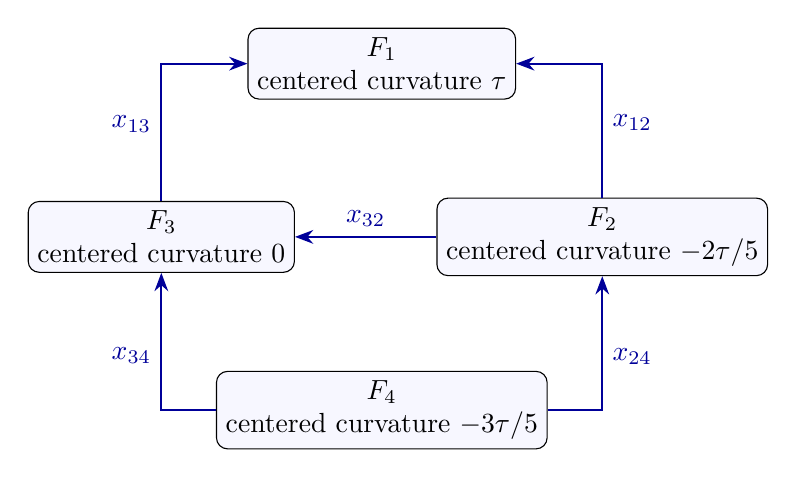
\begin{tikzpicture}[>=Stealth,
 vertex/.style={draw,rounded corners,fill=blue!3,
 minimum width=2.5cm,minimum height=.9cm,align=center},
 edge/.style={->,thick,blue!60!black}]
\node[vertex] (one) at (0,2.2) {$F_1$\\centered curvature $\tau$};
\node[vertex] (three) at (-2.8,0) {$F_3$\\centered curvature $0$};
\node[vertex] (two) at (2.8,0) {$F_2$\\centered curvature $-2\tau/5$};
\node[vertex] (four) at (0,-2.2) {$F_4$\\centered curvature $-3\tau/5$};
\draw[edge] (two.north) |- (one.east)
 node[pos=.28,right] {$x_{12}$};
\draw[edge] (three.north) |- (one.west)
 node[pos=.28,left] {$x_{13}$};
\draw[edge] (two.west) -- (three.east)
 node[midway,above] {$x_{32}$};
\draw[edge] (four.east) -| (two.south)
 node[pos=.70,right] {$x_{24}$};
\draw[edge] (four.west) -| (three.south)
 node[pos=.70,left] {$x_{34}$};
\end{tikzpicture}
\end{adjustbox}
\caption{The five allowed harmonic blocks on the unstable side.
Arrows run from source to target. For $\tau>0$ their line
quotients have the decreasing slope order $1,3,2,4$.
The full reconstruction also contains induced nonlinear entries;
the diagram does not replace the integrability equation $\kappa=0$.}
\label{fig:unstable-support}
\end{figure}


\subsection{The two-parameter scalar comparison}
For $a,d,q>0$ define
\begin{equation}\label{eq:logistic}
 \mathcal L_{a,d}(q,t;\tau)=
 \begin{cases}
 \displaystyle\frac{q e^{-a\tau t}}
 {1+\frac{dq}{a\tau}(1-e^{-a\tau t})},&\tau>0,\\[6pt]
 \displaystyle\frac{q}{1+dqt},&\tau=0.
 \end{cases}
\end{equation}
It solves $\dot z=-a\tau z-dz^2$, $z(0)=q$.
The expression is continuous at $\tau=0$ for each finite
time. Its denominator retains the independent initial energy
and distance from the wall.

\begin{theorem}\label{thm:signed-energy}
There are fixed $\tau_0,q_*>0$ such that, for
$0\le\tau\le\tau_0$ and integrable $x_0\in W$ with
$0<q_0=q_{-\tau}(x_0)<q_*$, the exact graph flow exists for
all $t\ge0$ and satisfies
\begin{equation}\label{eq:signed-energy}
 \mathcal L_{14/5,5}(q_0,t;\tau)\le q_{-\tau}(x(t))
                      \le\mathcal L_{2/5,1/5}(q_0,t;\tau).
\end{equation}
It preserves support and full integrability and reconstructs
an exact solution of \eqref{eq:flow}. The same assertion holds
on $d_{x_b}$ from any $x_0=e^{Y_0}x_b$ when both coefficient
presentations lie in the reconstruction domain. No bound
on $Y_0$ or ratio between $\tau$ and $q_0$ is required.
\end{theorem}
\begin{proof}
For $h=(3/2,-1/2,1/2,-3/2)$ one has $|h|^2=5$ and
$h_i-h_j\ge1$ on the five allowed blocks. Thus
$q_l/\sqrt5\le|\mu_l|\le\sqrt2q_l$.
The five characters of $b(-\tau)$, in order $12,13,32,24,34$,
are
\[
 -\tau(7/5,1,2/5,1/5,3/5).
\]
Consequently
$-7\tau q_l/5\le\langle\mu_l,b\rangle\le-\tau q_l/5$.
The exact energy derivative and the quartic remainder give
\[
 -\tfrac{14}{5}\tau q-4q^2-2\sqrt2C_Eq^3
 \le\dot q\le
 -\tfrac25\tau q-\tfrac25q^2+2\sqrt2C_Eq^3.
\]
Choose $q_*$ uniformly inside the signed graph domain and
with $2\sqrt2\max(C_E,1)q_*\le1/5$. Then
\begin{equation}\label{eq:signed-differential}
 -\tfrac{14}{5}\tau q-5q^2\le\dot q
                  \le-\tfrac25\tau q-\tfrac15q^2.
\end{equation}
The energy decreases, excluding exit from the smaller closed
coefficient ball. Smooth finite-dimensional continuation gives
every finite time; scalar exponential multipliers preserve
support and equivariance preserves $\kappa=0$. Comparison with
the two exact scalar solutions gives \eqref{eq:signed-energy}.
The reduced velocity is bounded on this region, so $Y$ and
$e^Y$ exist on every finite interval, allowing exact reconstruction.
\end{proof}

At $\tau=0$ this is the reciprocal estimate of
Theorem~\ref{thm:wall-energy}; at fixed positive $\tau$ it
gives exponential decay. The transition is uniform even when
$\tau/q_0$ tends to zero or infinity. Integrating the upper
profile also gives
\begin{equation}\label{eq:integrated-energy}
 \int_0^Tq_{-\tau}(x(t))\,dt\le
 \begin{cases}
 \displaystyle5\log\!\left(1+\frac{q_0}{2\tau}
                   (1-e^{-2\tau T/5})\right),&\tau>0,\\[5pt]
 5\log(1+q_0T/5),&\tau=0.
 \end{cases}
\end{equation}
The logarithmic derivative of the first denominator is one
fifth of the upper profile. Its infinite-time value is finite
for $\tau>0$, but can diverge as $\tau\to0$.
This distinction will determine the residual diagonal drift.

\begin{figure}[tbp]
 \centering
 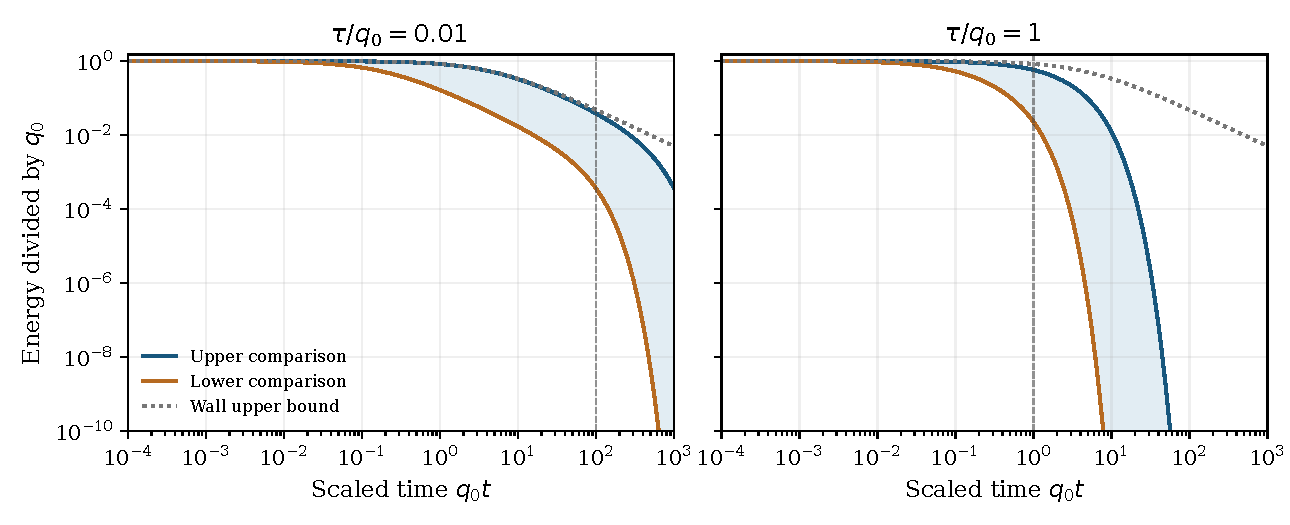
\includegraphics[width=.96\textwidth]{figures/fig02_transition.pdf}
 \caption{Exact scalar comparison profiles in
 \eqref{eq:signed-energy}. The horizontal variable is $q_0t$;
 the two panels use different values of the independent ratio
 $\tau/q_0$. Brown and blue curves are the lower and upper
 bounds; the gray dotted curve is the wall upper profile.
 The vertical dashed line marks $\tau t=1$.
 These are solutions of scalar comparison equations, not
 computed HYM trajectories.}
 \label{fig:transition}
\end{figure}

% Source: sections/05_phase.tex
\section{Phase with unbounded diagonal coordinates}\label{sec:phase}

We now allow complementary initial metric components. There
are two geometric domains: the full connected integrable nullcone
at $l=0$, and the connected triangular locus at $l=-\tau$,
$0\le\tau\le\tau_0$. The argument is shared, but the domain
at the wall is larger.

\subsection{Initial metrics and the energy cutoff}
Fix a small base tuple $x_b$ in one of these domains. For
$0<r\le r_0$ take
\begin{equation}\label{eq:initial-class}
 \begin{gathered}
 Y_0\in\mathfrak t_{\RR},\quad x_0=e^{Y_0}x_b,\quad
             0<q_0=q_l(x_0)<r^2/16,\\
 u_0\in\mathcal E_1,\quad v_0=u_0-\Psi(l,x_0),\quad
 \|v_0\|_{\mathcal E_1}<\delta,\quad
 D=\|v_0\|_{\mathcal E_\alpha},\qquad
 H^{\rm in}=e^{Y_0\,*}(h_0e^{u_0}).
 \end{gathered}
\end{equation}
Both $x_b$ and $x_0$ lie in the reconstruction domain.
There is no bound on $|Y_0|$, and no condition comparing $D$
with $r$. Uniform initial-data derivatives below concern
$(Y_0,v_0)$ with fixed $l,x_b$, not an unweighted matrix norm
on the original metric at an unbounded $Y_0$.

Put $x=e^Yx_b$ and $v=u-\Psi(l,x)$. Subtracting graph invariance
from \eqref{eq:normal-system} gives exactly
\begin{equation}\label{eq:phase-system}
 \begin{aligned}
 f(Y)&=\beta^\Psi(l,x),\\
 h(Y,v)&=\beta(l,x,\Psi(l,x)+v)-\beta^\Psi(l,x),\\
 F(Y,v)&=\mathcal N_l(x,\Psi+v)-\mathcal N_l(x,\Psi)
                            -D_x\Psi(l,x)C_xh(Y,v),\\
 \dot Y&=f(Y)+h(Y,v),\qquad \dot v=-A_lv+F(Y,v).
 \end{aligned}
\end{equation}
Choose a smooth $\chi:[0,\infty)\to[0,1]$, equal to one
on $[0,1]$ and zero on $[2,\infty)$. Multiply $f,h,F$ by
$\chi(q_l(e^Yx_b)/r^2)$ and extend them by zero.
Take $\sqrt2r$ within the common coefficient domain, using
uniform equivalence of $q_l$ and $|x|^2$, so extension occurs
before any reconstruction boundary. No Banach-norm cutoff
in $v$ is needed.

The diagonal characters give, for $j\le3$,
$|D_Y^jx|\le C_j|x|$ and $|D_Y^jq_l|\le C_jq_l$.
On the transition region $r^2\le q_l\le2r^2$, the first
two derivatives of the cutoff are consequently bounded
independently of $r,x_b,Y$. The exact first jets in
Section~\ref{sec:setup} give, on $\|v\|_{\mathcal E_\alpha}<\rho$,
\begin{equation}\label{eq:cutoff-estimates}
 \begin{aligned}
 \|f\|_{C^2}&\le C(\tau+r^2),\\
 \|D_vh\|+\|D_vF\|&\le C(r+\rho),\qquad
 \|D_vh(Y,v)\|\le C(r+\|v\|_{\mathcal E_\alpha}),\\
 \|D_Yh\|+\|D_YF\|&\le C\|v\|_{\mathcal E_\alpha},\qquad
 h(Y,0)=F(Y,0)=0.
 \end{aligned}
\end{equation}
Here $\tau=0$ for the full wall domain. All second derivatives
are bounded. For the normal bounds use the vanishing first
jets and $D_x\Psi C_x=O(r^2)$. Mixed derivatives and vanishing
at $v=0$ give the last line. Differentiating the cutoff
adds bounded factors multiplying maps already vanishing at
$v=0$. The first line must include $\tau$: cutoff derivatives
multiply the constant drift $b(-\tau)$.

Choose $\rho,r_0,\tau_0$ small enough for the criterion in
Section~\ref{sec:setup}, with $\|Df\|_\infty<c/8$, and then
choose $\delta$ uniformly for its initial and variation bounds.
For every smaller $r$ the same choices work. The cutoff system
has a global solution and a $C^1$ phase satisfying
\begin{equation}\label{eq:coordinate-phase}
 \begin{gathered}
 \|v(t)\|_{\mathcal E_\alpha}\le CD e^{-4ct},\qquad
 |h(Y(t),v(t))|\le C(r+D)D e^{-4ct},\\
 Y_{\rm ph}=\lim_{T\to\infty}\phi_{-T}(Y(T)),\qquad
 Y_*(t)=\phi_t(Y_{\rm ph}),\qquad
 |Y_*(t)-Y(t)|\le C(r+D)D e^{-4ct}.
 \end{gathered}
\end{equation}
The construction has used only bounded coefficients, with no
bound on the absolute diagonal coordinates. We next show
that both trajectories avoid the cutoff region.

\subsection{Perturbed energy confinement}
\begin{lemma}\label{lem:perturbed-energy}
After uniform reductions of $r_0,\delta$, both coefficient
trajectories stay in $q_l<r^2$ for all $t\ge0$ and retain
their initial support and integrability. For
$B\le C(r+D)D\le\log2$, the actual coefficient energy satisfies
\begin{equation}\label{eq:perturbed-energy}
 e^{-B}\mathcal L_{14/5,5}(q_0,t;\tau)\le q_l(x(t))
                \le e^B\mathcal L_{2/5,1/5}(q_0,t;\tau).
\end{equation}
For $q_*^0=q_l(x_*(0))$ the selected energy has the unforced
bounds \eqref{eq:signed-energy}, and
$|\log(q_*^0/q_0)|\le C(r+D)D$.
\end{lemma}
\begin{proof}
Before a first exit from $q_l<r^2$, the cutoff is one.
Diagonal equivariance preserves support and the full equation
$\kappa=0$. Theorems~\ref{thm:wall-energy} and
\ref{thm:signed-energy}, with $r^2<q_*$, give the corresponding
unforced energy inequality. Since $|\mu_l|\le\sqrt2q_l$,
the perturbation adds at most $\zeta(t)q_l$ in absolute value,
where $\zeta(t)=C(r+D)D e^{-4ct}$. Thus
\[
 -\tfrac{14}{5}\tau q-5q^2-\zeta q
 \le\dot q\le-\tfrac25\tau q-\tfrac15q^2+\zeta q .
\]
Let $B(t)=\int_0^t\zeta(s)\,ds\le B$.
For $z=e^{-B(t)}q$ and $w=e^{B(t)}q$,
\[
 \dot z\le-\tfrac25\tau z-\tfrac15e^{B(t)}z^2
            \le-\tfrac25\tau z-\tfrac15z^2,\qquad
 \dot w\ge-\tfrac{14}{5}\tau w-5e^{-B(t)}w^2
            \ge-\tfrac{14}{5}\tau w-5w^2 .
\]
Scalar comparison proves \eqref{eq:perturbed-energy}.
In particular $q_l(x(t))<2q_0<r^2/8$, excluding first exit.
Reduce $r_0,\delta$ so
$|Y_*-Y|_{\max}<1/4$. The diagonal character identity gives
$q_l(x_*)\le e^{4|Y_*-Y|_{\max}}q_l(x)<er^2/8<r^2$.
The selected trajectory therefore also sees no cutoff.
The exact reduced velocity remains bounded on each finite
time interval; no block disappears at finite time.
Applying the unforced theorem to that trajectory proves its
energy bounds. The same character estimate at time zero
gives the initial energy-ratio bound.
\end{proof}

Exact reconstruction now identifies both solutions with
actual metric flows on the original $d_{x_b}$:
\begin{equation}\label{eq:two-metrics}
 H(t)=e^{Y(t)\,*}(h_0e^{\Psi(l,x(t))+v(t)}),\qquad
 H_*(t)=e^{Y_*(t)\,*}(h_0e^{\Psi(l,x_*(t))}).
\end{equation}
The $\mathcal E_1$ initial class gives strong solutions, and
the first-jet parabolic realization gives positive-time
regularity. The nonlinear domain needs only the controlled
$\mathcal E_\alpha$ norm.

At the wall, integration of $|\dot Y|\le Cq_l+|h|$ and
\eqref{eq:perturbed-energy} gives
\begin{equation}\label{eq:actual-wall-drift}
 \begin{aligned}
 |Y(t)-Y_0|+|Y_*(t)-Y_{\rm ph}|
       &\le C\log(1+q_0t/5)+C(r+D)D,\\
 |Y(t)-Y_0|_{\max}
       &\ge\tfrac14\{\log(1+q_0t/5)-B\}.
 \end{aligned}
\end{equation}
For the selected trajectory the lower bound has $B=0$ and
$q_0$ replaced by $q_*^0$. Thus both diagonal increments
diverge, even though their difference tends to zero exponentially.

\subsection{Relative metrics and uniqueness}
Set $\Psi_*=\Psi(l,x_*(t))$ and define the relative positive
matrix in local $h_0$-unitary frames by
\begin{equation}\label{eq:relative-matrix}
 J_*(t)=e^{-\Psi_*/2}e^{-Y_*}(h_0^{-1}H(t))
                         e^{-Y_*}e^{-\Psi_*/2}.
\end{equation}
This congruence sends $h_0^{-1}H_*$ to the identity.
Writing $z=Y_*-Y$, the absolute diagonal cancels exactly:
\[
 J_*=e^{-\Psi_*/2}e^{-z}e^{\Psi(l,x)+v}e^{-z}e^{-\Psi_*/2}.
\]
The function $Y\mapsto q_l(e^Yx_b)$ is a sum of positive
exponentials and is convex. The segment between the two
diagonal coordinates therefore remains in $q_l<r^2$.
On it $\|D_x\Psi C_x\|_{\mathcal E_\alpha}\le Cr^2$, so
$\|\Psi(l,x)-\Psi_*\|_{\mathcal E_\alpha}\le Cr^2|z|$.
Smooth matrix functional calculus in the $h^{17/8}$
multiplication algebra now gives
\begin{equation}\label{eq:metric-tracking}
 \|\log J_*(t)\|_{h^{17/8}}\le\eta(t),\qquad
 e^{-\eta(t)}H_*(t)\le H(t)\le e^{\eta(t)}H_*(t),\qquad
 \eta(t)=CD e^{-4ct}.
\end{equation}
The logarithm is zero when $v=z=0$, and its derivatives
are bounded on the remaining small positive matrix neighborhood.
The estimate contains no condition number of $e^Y$.

\begin{lemma}\label{lem:inverse-metric}
For graph metrics $H_i=e^{Y_i\,*}(h_0e^{\Psi(l,e^{Y_i}x_b)})$
with both coefficient energies below $r^2$,
\begin{equation}\label{eq:inverse-metric}
 |Y_1-Y_2|\le C d_\infty(H_1,H_2).
\end{equation}
The constant is independent of the absolute $Y_i$.
\end{lemma}
\begin{proof}
Put $\Delta=Y_1-Y_2$ and $\Psi_i=\Psi(l,e^{Y_i}x_b)$.
Pull the order sandwich back by $e^{-Y_2}$ and take each
diagonal entry. If the order distance is at most $\eta$, this gives
\[
 |2\Delta_i+\log(e^{\Psi_1})_{ii}
                       -\log(e^{\Psi_2})_{ii}|\le\eta .
\]
The coefficient segment stays in $q_l<r^2$ by convexity.
Differentiating the scalar logarithm on that segment bounds
its difference by $Cr^2|\Delta|$. Taking the maximum and
using $|\Delta|\le2|\Delta|_{\max}$ absorbs the error after
shrinking $r_0$. These scalar diagonal entries are independent
of the choices of unitary line frames.
\end{proof}

The exact uncut field has derivative bounded by $Cr^2$
on this sublevel set: $b(l)$ is constant and the remaining
derivative is $O(q_l)$. Convexity gives the same Lipschitz
bound between any two endpoints there. If two graph flows
in this domain have order distance $O(e^{-ct})$ from $H$,
Lemma~\ref{lem:inverse-metric} bounds their coordinate
separation by the same exponential. Backward Gronwall on
each finite interval, with $Cr^2<c$, forces their initial
separation to be zero. This proves uniqueness in the stated
class and independence from the auxiliary cutoff, while
retaining dependence on the chosen graph.

\subsection{Initial-data regularity and spectra}
The strict inequalities in \eqref{eq:initial-class} define
an open metric class. Its normalization solves
$P_0\log(e^{-Y}(h_0^{-1}H)e^{-Y})=0$.
At a normalized $u$ the finite derivative is $-2R(u)$.
The pointwise multiplier of $S_u^{-1}C_u$ is
$a\coth a\ge1$, so $R(u)\ge I$. The implicit-function
theorem gives a smooth local inverse. At an arbitrary
$Y_0$, first pull back by $e^{-Y_0}$; the same calculation
has uniform bounds in that relative metric chart.
Integrating the positive derivative along a diagonal
segment proves uniqueness of the normalization.

The analytic phase criterion and
\eqref{eq:cutoff-estimates} show that $Y_{\rm ph}$ is $C^1$
in $(Y_0,v_0)$ at fixed $l,x_b$, with uniform bounds and
\[
 |Y_{\rm ph}-Y_0|\le C(r+D)D,\qquad
 \|D_{v_0}\Pi\|\le C(r+\delta),\qquad
 \Pi(Y_0,0)=Y_0 .
\]
These become initial-metric derivatives in the relative chart.
They do not assert uniformity for absolute matrix variations
at an unbounded diagonal.

\begin{theorem}\label{thm:local-tracking}
There are fixed $r_0,\tau_0,\delta,c,C,\gamma>0$ such that,
on either of the two domains stated at the start of this
section, every initial metric \eqref{eq:initial-class} selects
a reduced trajectory $x_*(t)=e^{Y_*(t)}x_b$ on the fixed graph
$\Psi$. Its initial value $Y_*(0)$ is $C^1$ in the relative
initial-metric coordinates at fixed $l,x_b$, and for all $t\ge0$
\[
 |Y_*(t)-Y(t)|\le C(r+D)D e^{-4ct},\qquad
 e^{-CD e^{-4ct}}H_*(t)\le H(t)\le e^{CD e^{-4ct}}H_*(t).
\]
The normal, energy and strong relative-logarithm estimates are
\eqref{eq:coordinate-phase}--\eqref{eq:metric-tracking}.
The selected trajectory is unique
among same-orbit graph trajectories in $q_l<r^2$ with
$d_\infty$ error $O(e^{-ct})$.

For the geometric spectra of $H,H_*$ and the finite spectrum
at $x_*(t)$, the kernels vanish and
\begin{equation}\label{eq:tracking-spectra}
 \begin{aligned}
 \left|\log\frac{\lambda_j(H(t))}{\lambda_j(H_*(t))}\right|
       &\le4CD e^{-4ct} &&(j\ge1),\\
 \left|\log\frac{\lambda_j(H(t))}{\nu_j(l,x_*(t))}\right|
       &\le Cq_l(x_*(t))+CD e^{-4ct} &&(1\le j\le3),\\
 \lambda_4(H(t))&\ge\gamma .
 \end{aligned}
\end{equation}
All constants are uniform in time, absolute diagonal
coordinates, support weights and positive spectral ratios.
\end{theorem}
\begin{proof}
Only the spectral assertions remain. Connected support and
the exact kernel in \eqref{eq:static-spectrum} give zero
trace-free holomorphic kernel. The sandwich
\eqref{eq:metric-tracking} compares squared endomorphism
norms in degrees zero and one by $e^{\pm2\eta}$; the
holomorphic differential is fixed. Min--max gives the first
line with $4\eta$. Pulling the graph metric to its
small-coefficient presentation is an exact isometry, even
when its diagonal is unbounded. Equation
\eqref{eq:static-spectrum} and the graph bound then give
the second line and fourth gap. Shrinking $r_0,\delta$
makes that gap uniform.
\end{proof}

At the wall $\lambda_3$ is comparable to
$q_*^0/(1+q_*^0t)$; on the unstable side it has the
corresponding two-sided scalar bounds, up to fixed factors.
No individual power or common exponential rate is inferred
for the smaller modes. For a nonzero disconnected support
the same proof applies with its exact $b-1$ dimensional
kernel: count the zeros, compare only positive indices,
and retain the fourth gap.

% Source: sections/06_entry.tex
\section{Entry from prescribed metrics}\label{sec:entry}

The local theorem imposes smallness on a complementary metric
component, but not on the diagonal factors. To reach that class
from a prescribed metric, we use a finite-time entry result
at the split reference object. The time is fixed before the
parameter and deformation neighborhoods are chosen.

\subsection{The finite-time input and its scope}
We use \cite[Proposition 6.2]{WuebbenPhase26} in the following
form. Let $H^0$ be any smooth positive metric on $E_0$ with
$\det H^0=\det h_0$, and put $W^0=\log(h_0^{-1}H^0)$.
There is $A>0$, depending on $H^0$ but not on the requested
tolerance, such that for every $\epsilon>0$ one can first
choose a finite time $T$, then positive signed-parameter
and coefficient radii and an open neighborhood $\mathcal U$
of $W^0$ in $h^{19/8}(\mathcal V)$, for which
\begin{equation}\label{eq:entry-input}
 H(T)=e^{Y_T\,*}(h_0e^{u_T}),\qquad
 |Y_T|_{\max}<A,\qquad P_0u_T=0,\qquad
 \|u_T\|_{h^{19/8}}<\epsilon .
\end{equation}
This holds for every small signed $l$, every complete
integrable $x_b$ in the resulting coefficient ball, and every
$W^{\rm in}\in\mathcal U$, with initial metric $h_0e^{W^{\rm in}}$
on $d_{x_b}$. The coordinates are normalized near a chosen
split-reference metric limit. They depend $C^1$ on the
initial metric, with uniform derivative bounds on these
finite-time neighborhoods. No stability hypothesis occurs.

The two ingredients matter here. On the split reference
bundle, order against $h_0$ bounds both the evolving metric
and its inverse. Smooth connection convergence modulo gauge,
as in the corrected \cite[Theorem 1.1(2)]{SibleyWentworth15},
then combines with elliptic estimates for the bounded
holomorphic convergence gauges to produce a metric subsequence
converging to a positive diagonal constant metric.
Second, the unsliced logarithmic metric equation has a common
normally elliptic principal part and smooth first-jet remainder.
Its strong $h^{19/8}$ finite-time map continues along the fixed
reference trajectory to the selected $T$.
The proof in \cite[Section 6]{WuebbenPhase26} verifies the
full-domain semiflow endpoint and the normalization derivative
$-2R(u)$. It neither differentiates an infinite-time limiting
metric nor requires a small positive finite spectral gap.

\subsection{The common-restart theorem}
\begin{theorem}\label{thm:prescribed}
Fix $H^0$ and the graph $\Psi$. There are
$A,C,c,\gamma,\epsilon_0>0$ such that, for every
$0<\epsilon<\epsilon_0$, one can choose a common finite
restart $T=T_\epsilon$, radii $\rho_\epsilon,r_\epsilon>0$,
a parameter bound $\tau_\epsilon>0$, and an open
$h^{19/8}$ neighborhood $\mathcal U_\epsilon$ of $W^0$
with the following properties.

The allowed data are either
\begin{equation}\label{eq:prescribed-domains}
 \begin{aligned}
 &l=0,\quad x_b\in\mathcal N^{\rm con}(\rho_\epsilon),\\
 &\text{or}\quad l=-\tau,\quad 0\le\tau\le\tau_\epsilon,\quad
                 x_b\in\mathcal Z_\triangle^{\rm con}(\rho_\epsilon),
 \end{aligned}
\end{equation}
and $W^{\rm in}\in\mathcal U_\epsilon$ in either case.
The flow from $H(0)=h_0e^{W^{\rm in}}$ has at $T$ the
normalization \eqref{eq:entry-input} and, with
$x_T=e^{Y_T}x_b$,
\begin{equation}\label{eq:entry-smallness}
 \begin{gathered}
 0<q_T=q_l(x_T)<r_\epsilon^2/16,\qquad
 v_T=u_T-\Psi(l,x_T),\\
 \|v_T\|_{h^{19/8}}<\epsilon,\qquad
 D_T=\|v_T\|_{h^{17/8}}\le\epsilon .
 \end{gathered}
\end{equation}
The time is chosen before the parameter, coefficient and
initial-metric neighborhoods.

For $s=t-T\ge0$, there are actual sliced coordinates and
a selected graph trajectory, both in $q_l<r_\epsilon^2$,
such that every conclusion of
Theorem~\ref{thm:local-tracking} holds with
$(Y_0,u_0,D,q_0,t)$ replaced by $(Y_T,u_T,D_T,q_T,s)$.
In particular
\begin{equation}\label{eq:prescribed-tracking}
 \begin{gathered}
 |Y_{\rm ph}-Y_T|\le C(\rho_\epsilon+D_T)D_T,\qquad
 \|\log J_*(s)\|_{h^{17/8}}\le CD_Te^{-4cs},\\
 e^{-CD_Te^{-4cs}}H_*(s)\le H(T+s)
                         \le e^{CD_Te^{-4cs}}H_*(s),\\
 \left|\log\frac{\lambda_j(H(T+s))}
                         {\nu_j(l,x_*(s))}\right|
       \le Cq_l(x_*(s))+CD_Te^{-4cs}\quad(1\le j\le3),\qquad
 \lambda_4(H(T+s))\ge\gamma .
 \end{gathered}
\end{equation}
The phase is unique in the same-orbit fast relative-metric
tracking class of that theorem. At each fixed $(l,x_b)$
it is $C^1$ in the initial metric on $\mathcal U_\epsilon$.
These derivative bounds may depend on $H^0,\epsilon$ but
are uniform over the chosen coefficient neighborhood.

All positive spectral ratios are unrestricted. In the
unstable domain no ratio between $\tau$ and coefficient
energy is restricted. No uniform restart over all prescribed
metrics is asserted.
\end{theorem}
\begin{proof}
Fix the local constants in Theorem~\ref{thm:local-tracking}
and choose $\epsilon_0<\delta/2$, with its other strict
normal margins. Apply the finite-time input to $H^0$
with tolerance $\epsilon/2$. It first gives $T$ and
$|Y_T|_{\max}<A$, then entry neighborhoods with
$\|u_T\|_{h^{19/8}}<\epsilon/2$.

Let $C_n$ bound $q_l(x)\le C_n|x|^2$ uniformly on the
signed entry interval. Shrink the parameter interval to
include the closed $[-\tau_\epsilon,0]$ within that interval
and within the local phase interval. Next choose
$\rho=\rho_\epsilon$ so small that, with
\begin{equation}\label{eq:entry-radii}
 r=8\sqrt{C_n}e^{2A}\rho,
 \qquad r\le r_0,\qquad
 C_\Psi C_ne^{4A}\rho^2<\epsilon/2 ,
\end{equation}
the coefficient ball also lies inside the entry neighborhood.
The diagonal action gives
$q_l(e^{Y_T}x_b)\le C_ne^{4A}|x_b|^2<r^2/64$.
The graph norm is below $\epsilon/2$, proving
\eqref{eq:entry-smallness}. Keep or shrink the metric
neighborhood provided by the entry theorem.

Diagonal action preserves both geometric domains, their
support and the complete obstruction equation. The local
tracking theorem therefore applies at $T$. Its exact
reconstruction agrees with the prescribed metric there;
uniqueness of the parabolic flow identifies the all-future
solution. Its phase and coordinate bounds
$C(r+D_T)D_T$ become $C_{H^0}(\rho+D_T)D_T$ by
\eqref{eq:entry-radii}. The energy estimates are precisely
\eqref{eq:perturbed-energy} and the unforced bounds at the
selected initial energy. This proves all assertions in
\eqref{eq:prescribed-tracking}, including the strong norm
at $s=0$. The all-positive spectral comparison of the
local theorem also applies.

At the fixed finite $T$, the restart map is $C^1$ uniformly
on the chosen ambient neighborhoods. Subtracting
$\Psi(l,e^{Y_T}x_b)$ adds the derivative
$D_x\Psi C_x=O(q_T)$. Compose with the $C^1$ phase map
already proved on the coefficient sublevel set. This gives
the initial-metric derivative assertion without differentiating
the split-reference limit or an inverse weak eigenvalue.
\end{proof}

The theorem compares actual flows from $T$ onward. The finite
entry result controls the preceding interval; a backward
parabolic problem is never solved. For smooth initial metrics
the solution is smooth. The stated strong neighborhood also
permits $h^{19/8}$ initial data with the full-domain local
regularity and positive-time regularity used in the proof.
At $\tau=0$, both descriptions agree on their common triangular
subspace by uniqueness of the selected phase for the fixed graph.

% Source: sections/07_residual.tex
\section{Residual drift and the graded connection}\label{sec:residual}

On the unstable side, integrability of the coefficient energy
allows subtraction of the linear diagonal drift. The remaining
constant retains finite initial data. At the wall the same
energy integral diverges, and this residual need not exist.

\subsection{The residual for an exact graph trajectory}
\begin{theorem}\label{thm:residual}
Fix $0<\tau\le\tau_0$ and a connected integrable triangular
base $x_b$ in the reconstruction domain.
For an exact graph trajectory from $Y_0$ with
$q_0=q_{-\tau}(e^{Y_0}x_b)<q_*$, the limit
\begin{equation}\label{eq:residual-integral}
 Z_\infty=\lim_{t\to\infty}(Y(t)-b(-\tau)t)
 =Y_0+\int_0^\infty
          \{\beta^\Psi(-\tau,x(t))-b(-\tau)\}\,dt
\end{equation}
exists. With uniform $C_\beta$,
\begin{equation}\label{eq:residual-bounds}
 \begin{aligned}
 |Z_\infty-Y_0|&\le5C_\beta\log(1+q_0/(2\tau)),\\
 |Z_\infty-(Y(t)-b(-\tau)t)|
       &\le5C_\beta\log(1+q_{-\tau}(x(t))/(2\tau))
        \le\frac{5C_\beta}{2\tau}q_{-\tau}(x(t)).
 \end{aligned}
\end{equation}
On the open initial set $q_{-\tau}(e^{Y_0}x_b)<q_*$,
the map $Y_0\mapsto Z_\infty$ is $C^1$ and a local
diffeomorphism, with
\begin{equation}\label{eq:residual-derivatives}
 \|D_{Y_0}Z_\infty\|+
 \|(D_{Y_0}Z_\infty)^{-1}\|
       \le2(1+q_0/(2\tau))^C .
\end{equation}
Every active harmonic block has the nonzero limit
\begin{equation}\label{eq:rescaled-blocks}
 e^{-(b_i-b_j)t}x_{ij}(t)
       \longrightarrow
 e^{(Z_\infty)_i-(Z_\infty)_j}(x_b)_{ij}.
\end{equation}
\end{theorem}
\begin{proof}
The exact field satisfies $|\beta^\Psi-b|\le C_\beta q_l$.
Equation \eqref{eq:integrated-energy} gives absolute convergence
of \eqref{eq:residual-integral} and its first bound.
Apply that same estimate to the autonomous trajectory
restarted at time $t$ to bound the tail; $\log(1+s)\le s$
gives the last inequality. The block limit is the exact
character identity $x_{ij}=e^{Y_i-Y_j}(x_b)_{ij}$.

Write $f(Y)=\beta^\Psi(-\tau,e^Yx_b)$. The moment derivative
is $O(q_l)$, and the differentiated quartic remainder,
composed with $D_Yx=C_x=O(|x|)$, is $O(q_l^2)$.
Therefore $\|Df(Y)\|\le Cq_l(e^Yx_b)$ along the invariant
region, independently of $|Y|$. For the finite variational
matrix $J(t)=D_{Y_0}Y(t)$,
\[
 \dot J=Df(Y(t))J,\qquad J(0)=I,\qquad
 \|J(t)\|,\|J(t)^{-1}\|
       \le\exp\!\left(C\int_0^tq_l(x(s))\,ds\right).
\]
At fixed $\tau>0$ this integral is finite. Both $\dot J$
and the derivative of $J^{-1}$ are integrable, so the
matrices have limits whose product is the identity.
The integrated energy bound yields
\eqref{eq:residual-derivatives}.

To identify the limit as a derivative, take a small compact
neighborhood of $Y_0$ within the open energy region.
There its initial energy is at most some $\bar q<q_*$,
and $q_l(x(t))\le\bar q e^{-2\tau t/5}$ uniformly.
The residual integrals and their first variations thus
converge locally uniformly. Their limits are $C^1$ and
have the invertible derivative just obtained. The
inverse-function theorem proves local invertibility.
Connected support removes the trace-free diagonal stabilizer,
so these are three independent initial diagonal coordinates.
\end{proof}

For an actual solution of Theorem~\ref{thm:local-tracking},
apply this theorem to its selected trajectory. Since
$Y_*-Y_{\rm act}\to0$ exponentially, both residuals have
the same limit. In the prescribed-entry notation,
\[
 |Z_\infty-Y_T|
 \le C(\rho_\epsilon+D_T)D_T
            +5C_\beta\log(1+q_*^0/(2\tau)).
\]
The actual tail has, in addition to the selected tail in
\eqref{eq:residual-bounds}, the term
$C(\rho_\epsilon+D_T)D_Te^{-4cs}$.
Both rescaled actual and selected blocks have the limits
\eqref{eq:rescaled-blocks}, with time measured from restart.
Composition with the phase and restart maps proves $C^1$
dependence on the prescribed initial metric at fixed
$\tau>0,x_b$. The local invertibility assertion concerns the
three real diagonal initial coordinates of the reduced flow.

Neither the residual nor its derivative is bounded uniformly
as $\tau\to0$ by these estimates. At the wall,
\eqref{eq:actual-wall-drift} forces unbounded diagonal
displacement for nonzero data. Figure~\ref{fig:residual-bound}
shows the integral bound that distinguishes the two regimes.

\begin{figure}[tbp]
 \centering
 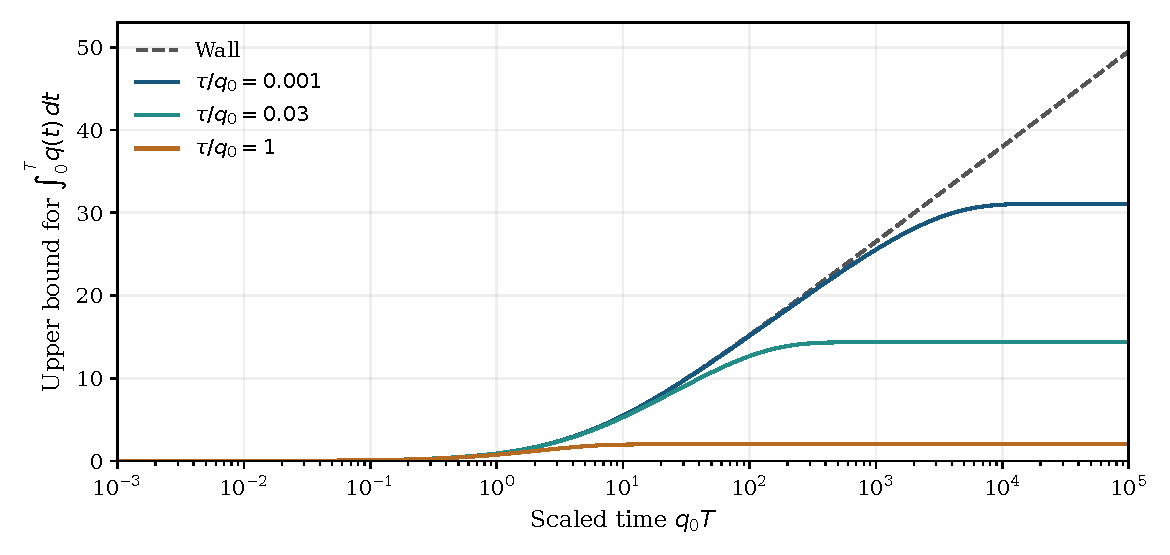
\includegraphics[width=.75\textwidth]{figures/fig03_residual_bound.pdf}
 \caption{The integral of the upper scalar energy profile in
 \eqref{eq:integrated-energy}, as a function of $q_0T$.
 Positive values of $\tau/q_0$ give finite limits; the wall
 curve grows logarithmically. Multiplication by $C_\beta$
 bounds displacement after subtracting linear drift.
 The curves are exact comparison integrals, not actual
 residual trajectories.}
 \label{fig:residual-bound}
\end{figure}

\subsection{An explicit topology for convergence of connections}
Let $A_H(t)$ be the Chern connection on $(d_{x_b},H(t))$,
and write its actual coordinates as
$u(t)=\Psi(l,x_{\rm act}(t))+v(t)$.
The isometry from this evolving metric to $h_0$ is
\begin{equation}\label{eq:moving-isometry}
 U(t)=e^{u(t)/2}e^{Y_{\rm act}(t)},\qquad
 U(t)^*h_0U(t)=H(t).
\end{equation}
Here the first factor is the positive isometry in the
small-coefficient presentation; the order of factors matters.

\begin{proposition}\label{prop:graded-limit}
For every local trajectory above, or from the common restart
in Theorem~\ref{thm:prescribed}, the transported connection
$\widetilde A(t)$ satisfies
\begin{equation}\label{eq:connection-limit}
 \|\widetilde A(t)-A_0\|_{h^{9/8}}
 +\|F_{\widetilde A(t)}-F_{A_0}\|_{h^{1/8}}
       \le C\bigl(q_l(x_{\rm act}(t))^{1/2}+D e^{-4ct}\bigr)
       \longrightarrow0 .
\end{equation}
For $\tau>0$, $A_0$ is the split HN graded connection;
at the wall it is the equal-slope HE graded connection.
There is no curvature concentration in these flows.
\end{proposition}
\begin{proof}
Transport first by $e^{Y_{\rm act}}$. Exact reconstruction
equivariance gives the Chern connection of $(d_x,h_0e^u)$;
there is no norm or spatial derivative of the large diagonal
left to estimate. Relative to $A_0$, its $(1,0)$ part is
\[
 e^{-u}\nabla_0^{1,0}e^u-e^{-u}a(x)^{*h_0}e^u .
\]
The additional isometry $e^{u/2}$ involves a smooth matrix
function and one spatial derivative of $u$. Hence its
connection difference $B$ has
$\|B\|_{h^{9/8}}\le C(|x|+\|u\|_{h^{17/8}})$.
The reconstruction has bounded higher spatial norms on its
coefficient ball, and
$\|u\|_{h^{17/8}}\le Cq_l(x)+CD e^{-4ct}$.
Uniform norm equivalence and $q_l(x)<1$ give the first
bound in \eqref{eq:connection-limit}.

For the curvature use
$F_{A_0+B}-F_{A_0}=d_{A_0}B+B\wedge B$.
A derivative sends $h^{9/8}$ to $h^{1/8}$ and multiplication
is continuous in these spaces. The same bound follows for
the curvature. The energy estimates tend to zero in both
regimes. Proposition~\ref{prop:hn-filtration} and
Proposition~\ref{prop:wall-geometry} identify the limiting
graded bundle. Each factor's product metric is HE for
$\omega_l$, though the four mean curvatures are unequal
when $\tau>0$. Uniform curvature convergence in these
isometries excludes concentration.
\end{proof}

After the usual positive identification of $H(t)$ with
$h_0$, the difference from \eqref{eq:moving-isometry} is
unitary. Thus this also gives convergence modulo unitary
gauge for that fixed-metric connection family. The assertion
is in the displayed H\"older topologies and uses a
time-dependent unitary gauge.

\FloatBarrier
\begin{thebibliography}{Wue26d}

\bibitem[HKKP18]{HKKP18}
F.~Haiden, L.~Katzarkov, M.~Kontsevich and P.~Pandit,
\emph{Iterated logarithms and gradient flows}, preprint, 2018,
\href{https://arxiv.org/abs/1802.04123v1}{arXiv:1802.04123v1}.

\bibitem[Kob87]{Kobayashi87}
S.~Kobayashi, \emph{Differential Geometry of Complex Vector Bundles},
Publications of the Mathematical Society of Japan, vol.~15,
Kan\^o Memorial Lectures, vol.~5, Iwanami Shoten and Princeton
University Press, 1987.
\href{https://www.mathsoc.jp/assets/pdf/publications/pubmsj/Vol15.pdf}
{Official Mathematical Society of Japan edition}.

\bibitem[Lam26]{Lam26}
S.~T.~Lam, \emph{Semistability and asymptotics of geometric flows},
preprint, 2026,
\href{https://arxiv.org/abs/2606.09235v1}{arXiv:2606.09235v1}.

\bibitem[SW15]{SibleyWentworth15}
B.~Sibley and R.~A.~Wentworth,
\emph{Analytic cycles, Bott--Chern forms, and singular sets for
the Yang--Mills flow on K\"ahler manifolds},
Adv. Math. \textbf{279} (2015), 501--531.
\href{https://doi.org/10.1016/j.aim.2015.04.009}
{doi:10.1016/j.aim.2015.04.009}.
The corrected text and appended erratum are
\href{https://arxiv.org/abs/1402.3808v3}{arXiv:1402.3808v3}.

\bibitem[Wue26a]{WuebbenThreeStep26}
B.~J.~Wuebben, \emph{Hermitian--Einstein metrics and small spectra
for three-step extensions}, preprint, October 31, 2026.
\href{https://doi.org/10.5281/zenodo.23850990}{doi:10.5281/zenodo.23850990}.

\bibitem[Wue26b]{WuebbenPhase26}
B.~J.~Wuebben, \emph{Initial conditions and asymptotic phase
for Hermitian--Yang--Mills flow}, preprint, October 31, 2026.
\href{https://doi.org/10.5281/zenodo.23850996}{doi:10.5281/zenodo.23850996}.

\bibitem[Wue26c]{WuebbenFlow26}
B.~J.~Wuebben, \emph{Metric response and Hermitian Yang--Mills
flow for two-step extensions}, preprint, October 27, 2026.
\href{https://doi.org/10.5281/zenodo.23717742}
{doi:10.5281/zenodo.23717742}.

\bibitem[Wue26d]{WuebbenWall26}
B.~J.~Wuebben, \emph{$L^2$ metrics on Hermitian--Yang--Mills moduli spaces near a stability wall},
preprint, October 31, 2026.
\href{https://doi.org/10.5281/zenodo.23850992}{doi:10.5281/zenodo.23850992}.

\end{thebibliography}

\end{document}
